
% Zitat: Auf den Schultern von Riesen.

This chapter will give an introduction into the basics needed to
understand this thesis. First, an introduction into functional programming
in Haskell is given - it is to ease the understanding of the code involved.
Then Nested Data Parallelism (NDP) is covered where
key insights are made and concepts that exploit them are presented.
Afterwards a short introduction into parallel complexity measures is given.
The concept of work and depth complexities are given
- together with definitions to calculate them.
Finally, \algo is presented. Its problem is described and
the solution is formulated.

\section{Haskell}
  Haskell is a general-purpose strongly-typed purely-functional programming
  language. It has full type-inference, referential transparency, higher-order-functions
  and more features. Functional programming in Haskell and similar languages
  is guided by two ideas - "write what you mean" and "let the compiler do the work for you".
  The former means the use of high abstractions to write concise code -
  while the latter means the use of sophisticated compilers
  \footnote{some which - like the Glasgow Haskell Compiler - are written in Haskell themselves}
  to optimise the abstractions to efficient machine code.
  
  A few of the main features needed in this thesis are presented now:
  
  
  \paragraph{Syntax}
    Consider this function:
    \begin{lstlisting}
foo :: Double -> Int
foo x = round (max 5 x)
    \end{lstlisting}
    \c{foo} takes the maximum of 5 and the argument number \c{x} and
    rounds it to the nearest integer. The function is given a type
    signature in the first line. \c{f :: t} denotes that \c{f} is of type \c{t}.
    The type describes a function from a double floating number
    to an integer. Multiple argument functions are typed with multiple arrows.
    E.g. \c{max :: Double -> Double -> Double}-
    In contrast to many programming languages parentheses \c{()} are not used for function application
    (as in \c{f(a)}) but instead are used to specify precedence/ordering.
    Function application is expressed with spacing - space as in ' '. E.g. \c{round 5.2} applies the built-in
    floating point rounding function to return the integer \c{5}. Multiple-argument
    functions are be applied with multiple spaces. E.g. \c{max 5 x}
    applies \c{max} on \c{5} and \c{x}.
    
    The function is written alternatively as:
    \begin{lstlisting}
foo :: Double -> Int
foo x = let a = max 5 x
                  b = round a
            in  b
    \end{lstlisting}
    \c{let} statements bind expressions to variables.
    The expression after the \c{in} keyword is the return value of the
    entire expression.
    
    The function can be written without the explicit use of its argument \c{x}.
    \begin{lstlisting}
foo = (round) . (max 5)
foo = round . max 5
    \end{lstlisting}
    This is called currying and function composition.
    One can omit the last argument of a function and define the function
    \c{foo} and focus on the functionality: "Take the maximum of 5 and then round".
    Function composition is denoted by a dot \c{(.)}.
    The second line shows, that the space operator binds stronger than function composition.
    
    In functional programming one often ends up nesting multiple functions:
    \begin{lstlisting}
myFunc x = (bar a b (baz c (foo d x)))
    \end{lstlisting}
    One can write the same function in various different ways - depending on space
    and visual ease.
    \begin{lstlisting}
myFunc x = bar a b . baz c . foo d $ x  -- composed with explicit argument
myFunc = bar a b . baz c . foo d        -- composed with implicit argument
myFunc x = bar a b                      -- indented, explicit argument
               . baz c 
               . foo d
               $ x
myFunc = bar a b                        -- indented, implicit argument
             . baz c
             . foo d
    \end{lstlisting}
    The new \c{\$} operator is used here. It denotes function application either.
    % \footnote{Fun fact: \c{\$} is defined in Haskell itself! It goes by \c{f \$ x = f x}}
    However, it
    has very low precedence - so that the functions are composed first
    before the argument is applied into the pipeline of functions.
    The reader is noted, that the multi-line definitions actually apply
    the functions from bottom to up. First foo, then baz
    and finally bar is applied - even though foo is written last.
    
  \paragraph{Naming Conventions}
    Higher order functions are denoted with \c{f},\c{g} or \c{h}.
    Variables are denoted with \c{x},\c{y},\c{z},\c{a},\c{b},\c{c}
    or with longer names like \c{divisor} or \c{multWith2}.
    Two closely related variables are given
    primes. E.g. they are named \c{x} and \c{x'}. A prime is a part of the variable name.
    Finally, a collection of \c{x} will be referred to by \c{xs}.
    E.g. \c{xs} is an array, \c{xss} is a two dimensional array, and so on.
  
  \paragraph{Strong typing and Type Inference}
    Every expression has a type. A program containing
    ill-typed expressions, e.g. \c{3 + False}, is rejected.
    Types can be (almost always) be inferred from the context and
    don't need to be specified.
    
  \paragraph{Type Synonyms}
    Type synonyms enable one to refer to a complicated type by a simpler name.
    E.g. \c{type Foo a = (Int,a)} defines a type synonym - such that
    \c{Foo Double} is replaced by \c{(Int,Double)} during compilation.
  
  \paragraph{Referential Transparency and Immutability}
    Functions and expressions are referentially transparent in Haskell.
    Like their inspiring equivalent in Mathematics, they always return
    the same result when evaluated (with the same arguments).
    A consequence is Immutability - variables and data structures
    cannot be mutated. Functions over data structures return
    new copies instead of mutating the argument. This enables
    powerful optimization techniques such as Inlining and Rewrite Rules.
    They are explored in section \ref{section:ndpintro}.
    
  \paragraph{Record Syntax}
    Records combine multiple values into a single complex value.
    The following snippet creates a record of type \c{Person} with the
    fields \c{name} and \c{age}.
    \begin{lstlisting}
Person {
  name = "Mark"
  age = 23
}
    \end{lstlisting}
    
  \paragraph{Polymorphism}
    Types can be polymorphic. 
    E.g. one can write the following general function
    without nesessarily fixing to concrete types.
    \begin{lstlisting}
foo :: a -> b -> a
foo x y = x
    \end{lstlisting}
    Lower case letters in the type signature denote type variables.
    This function is well-defined for both arguments
    as long as the return type is same as the type of \c{x}. This
    restriction is reflected in the type signature - the first and
    the last type variable have to be equal. 
    
    Similarly, one can define functions over polymorphic data types.
    E.g. \c{List a} denotes a list of elements of type a. \c{List Int}
    is by that definition a linked list of integers.
    
    Polymorphisim is for example useful in \c{map :: (a -> b) -> List a -> List b}.
  
  \paragraph{Higher Order Functions}
    Functions are values and can be taken or passed ar arguments to other functions.
    \c{map} is an example.
    \begin{lstlisting}
map :: (a -> b) -> List a -> List b
    \end{lstlisting}
    Given a function from \c{a} to \c{b} and a List of \c{a}-typed values,
    \c{map} applies the function on every element and produces a List
    of \c{b}-typed values.
    
  \paragraph{Lambdas}
    Functions can be written literally using Lambda expressions.
    For example, the function \c{f x = 2*(x+1)} can be written
    directly as \c{f = \lam x -> 2*(x+1)} or \c{f = \textbackslash{x} -> 2*(x+1)}.
    The backslash \textbackslash{} is used inside code snippets - \lam{} is used outside of them.
    \footnote{The \textbackslash{} is used because of its similarity to \lam.}
    
  \paragraph{Identity, flip and function composition}
    Three commonly used functions are:
    \begin{lstlisting}
id :: a -> a
id x = x
flip :: (a -> b -> c) -> b -> a -> c
flip f x y = f y x
(.) :: (b -> c) -> (a-> b) -> a -> c
g . f = \x -> g (f x)
    \end{lstlisting}
    \c{id} is the identity function and \c{flip} exchanges a functions
    first two arguments.
    The identity function is the neutral element of function composition \c{(.)}
    and the following law holds:
     \c{\textrm{$\forall$} f: f . id = id . f = f}. This is useful for Rewrite Rules.


  \p
  A brief overview has been given. An introduction to Nested Data Parallelism is given next.



\section{Nested Data Parallelism}
  \label{section:ndpintro}
  
  In the ground breaking work \cite{Belloch1996}
  major contributions to parallel programming in
  functional programming languages were made.
  The paper presented some of Belloch's earlier work (\cite{NepaBelloch1993}) on NESL
  - a programming language specifically designed for expressing parallelism
  in functional programming languages. Its ideas and insights were
  adapted to various languages - one of them being Haskell.
  Multitude years of research generalized the
  results of the special purpose language NESL
  to the widely general purpose language Haskell.
  \footnote{For example \cite{Harness2008}, \cite{DPHStatus2007},
  \cite{EffiVect2012Lipp}, \cite{HighOrdFlat2006} and \cite{DistTypes1999}.}
  This project is called Nested Data Parallel Haskell and this section will give
  an overview of its key concepts.
  
  \paragraph{}
    In Flat Data Parallelism, the programmer is provided with parallel mapping primitives
    to express parallelism. Such a function might be \c{map} such that \c{map f xs} applies \c{f}
    on each of the elements in the array \c{xs} in parallel.
    
    This function has a fairly intuitive parallel implementation:
    First distribute the input array evenly across the \underline{p}rocessing \underline{u}nits (PUs),
    then compute each local chunk of the array with its PU and finally join all elements together.
    The inner function \c{f} is applied by each processing unit (PU) sequentially.
    
    Statements like \c{map incr}
    \footnote{\c{incr :: Int -> Int} increments an integer.}
    can be perfectly parallelized.
    However, one comes it its limits when considering statements like \c{map (map incr)} or \c{map (map (map incr))}.
    Within Flat Data Parallelism only the outer-most level is run in parallel.
    Running the inner elements in parallel requires a different approach in dividing up the workload.
    
    \p
    Nested Data Parallelism lifts these limitations.
    In NDP \c{f} can be a parallel operation either. All levels of nesting can
    be executed in parallel - hence the name: \textbf{Nested} Data Parallelism.
    It achieves this by transforming the source program into a functionally
    equivalent flat data-parallel program. This (non-trivial) transformation
    is called 'Flattening' or 'Vectorization' and includes subsequent compiler optimisations.
    
    The entire program transformation can be broken down in three steps.
    Each step introduces its new data types. They are presented below:
    \begin{enumerate}
      \item \emph{Vectorization} -
        The nested arrays \pan{} which are used by the programmer
        are converted to flat type-dependent array representations - namely  \pav{}.
        The flattening is also applied to nested parallel functions like
        those mentioned in the previous paragraph.
      \item \emph{Communication Fusioning} -
        By inlining the definitions of the parallel functions and
        using semantics-preserving rewrite rules one can
        reduce unnecessary synchronisation points and
        create tight processing pipelines. It uses \pad{} to denote
        distributed chunks of the global array \pav{}.
      \item \emph{Stream Fusioning} -
        Sequential functions local to each PU can further
        be optimised to reduce the number of intermediate arrays
        and to create tight loops.
        It uses \type{Vector a} and \c{Stream a} to
        implement the local array chunks and to fuse loops, respectively.
    \end{enumerate}
    
  \p
  For parallel arrays, one has few predefined functions.
  They correspond to functions used in conventional functional programming.
  Their names and their types are given in \ref{table:parfuns}.
  \footnote{e.g. \c{zipWithP (*) [:1,2,3:] [:1,3,4:] = [:1*1,2*3,3*4:]}. The arrays as assumed to be of equal size.}
  \begin{table}[h]
    \caption{Parallel functions in NDP}
    \label{table:parfuns}
    \begin{tabular}{lll}
        \toprule
        function & type & description \\
        \midrule
        (!:),indexP & \c{[:a:] -> Int -> a} & indexes the array \\
        lengthP & \c{[:a:] -> Int} & returns the length of the array \\
        headP & \c{[:a:] -> a} & returns the first element\\
        lastP & \c{[:a:] -> a} & returns the last element \\
        mapP & \c{(a -> b) -> [:a:] -> [:b:]} & applies a function on all elements \\
        zipWithP & \c{(a -> b -> c)} & zip together pairs of elements by \c{f} \\
         & \c{-> [:a:] -> [:b:] -> [:c:]} & and return an array of results \\
        sortP & \c{[:Int:] -> [:Int:]} & sorts an array \\
        sumP & \c{[:Int:] -> Int} & sums the arrays elements \\
        concatP & \c{[:[:a:]:] -> [:a:]} & removes a level of nesting \\
        unconcatP & \c{[:[:a::]] -> [:b:] -> [:[:b:]:]} & exposes a structure to a flat array \\
        replP & \c{Int -> a -> [:a:]} & replicates an element \\
    \end{tabular}
  \end{table}
    
  \subsection{Vectorization}
    Vectorization involves two major steps -
    \emph{Type dependent representation} and \emph{Lifting}.
    Both will be explained in detail below.
  
    \subsubsection{Type dependent representation}
      Type dependent representation enables the programmer
      to work with arrays containing complex
      data structures without scarifying efficiency.
      It is described in 
      \cite{FastArr2003Chakravarty}
      and \cite{DataFamily2005Chakravarty}.
      
      Consider for example \type{[:Int:]} and \type{[:[:Int:]:]}.
      The former can be easily implemented using a contiguous region
      of memory and inserting the bytes. The latter however cannot
      be implemented equally. The sub-array could be of different size.
      To allocate a block of memory, one needs to know the size of all arrays beforehand.
      Implementing nested array naively would use an array of pointers to
      to arrays of integers. Pointers however are undesirable, since they
      decrease Cache Locality. CPU Caching is crucial for performance
      and is directly linked to Cache Locality.
      
      Nested arrays need a different approach for representation.
      That approach is the separation of data and structure.
      The following example describes how a nested array
      like \c{[[1,2,3],[4,5],[],[6]] :: [:[:Int:]:]} can be implemented
      to increase Cache Locality:
      \footnote{\c{[\string#1,2,3\string#]} is the notation used for a contiguous-memory array.}
      \begin{lstlisting}
array :: PA (PA Int)
array = AArr {
  data = [# 1,2,3,4,5,6 #],
  indices = [# 0,3,5,5 #]
  lengths = [# 3,2,0,1 #]
}
      \end{lstlisting}
      All data is packed together into a data field - regardless of nesting.
      All structural information is divided into two arrays of integers.
      The indices-array contains - for every subarray in the 
      original array - the index of the first element if it were
      to be indexed into the \c{data} field. The lengths describe the lengths of
      each sub-array. Each sub-array corresponds to a pair of index and length.
      For example, the \underline{second} sub-array (\c{[4,5]}) corresponds to
      the \underline{second} index (3) and \underline{second} length (2). Extracting
      2 elements starting at index 3 in the \c{data} array will return
      exactly these two elements.
      
      This flat representation uses the new type \type{PA (PA Int)}
      instead of the old \type{[:[:Int:]:]}. 
      For nested arrays the functions \c{concatP} and \c{unconcatP}
      become constant time operations. Removing a level of nesting
      is as simple as discarding the segment descriptors.
      Adding a nesting structure of an existing array to a flat array
      is implemented by adding the segment descriptor of the nested array to the
      flat array.
      
      The flat representation of irregularly nested arrays
      and the constant time (un-)flattening operations are crucial insights in
      NDP.
      
      Implementation for all other types - such as arrays of ints,
      arrays of doubles, are also given. For example \c{[:1,2,3:] :: [:Int:]} can be simply
      represented as:
      \begin{lstlisting}
array :: PA Int
array = AInt [# 1,2,3 #]
      \end{lstlisting}
      
      Finally, during flattening the compiler transforms
      every parallel functions (like \c{fooP}) to
      their predefined scalar counterparts (like \c{fooPS}).
      The scalar functions work directly on the flat representation
      and are designed to exploit them for efficiency.
      \c{concatPS} and \c{unconcatPS} are examples thereof.
      In fact, functions like \c{fooP} have no actual implementation
      because they are entirely replaced by their \c{fooPS} counterparts.
      They are solely used to simplify the programmer view.
    
    \nomenclature{Cache Locality}{TODO}
      
    \subsubsection{Lifting}
      During lifting where all occurrences of \c{mapPS f} are
      replaced by \c{fL} and where \c{fL}
      is the lifted version of the original function.
      Compared to the original scalar function \c{f :: a -> b}, the lifted
      function applies the mapping over arrays. It is given by \c{fL :: PA a -> PA b}.
      For user-defined functions, the lifted function is defined by lifting the definition of \c{f} recursively.
      The key is now the definition of the lifted functions for the built-in functions.
      The most important one among them is lifted \c{mapPS} - namely \c{mapPL}.
      To \c{mapPS} of type \c{(a -> b) -> PA a -> PA b},
      \c{mapPL} is of type \c{(a -> b) -> PA (PA a) -> PA (PA b)}.
      To overcome the limitations of flat data parallelism,
      its implementation has to map over all elements at once
      (instead of mapping over the outer-nesting level only).
      The following implementation does that.
    \begin{lstlisting}
mapPL :: (a -> b) -> PA (PA a) -> PA (PA b)
mapPL f xss =
  unconcatPS xss
  . fL
  . concatPS
  $ xss
    \end{lstlisting}
    The definition of \c{mapPL} is curcial.
    First it flattens the array (line 5), then it applies
    the flat data-parallel operation (line 4) using \c{fL}
    and finally the array is un-flattened to the original structure (line 3).
    \footnote{This implementation is different from the original in one important aspect - 
    namely the handling of pre-supplied arguments in the function. Our
    implementation only handles functions without pre-supplied arguments -
    but it much simpler to understand than the original in
    in \cite{HighOrdFlat2006}.
    More accurately, one has an additional expression \c{expandPS xss fEnv}.
    Introducing it wouldn't affect the overall situation in this thesis.
    Therefore, it was omitted.
    } 
    Figure \ref{figure:mapP} shall visually aid the understanding
    using the example \c{mapP (mapP incr)}.
    
    \begin{figure}[h!]
        \begin{center}
        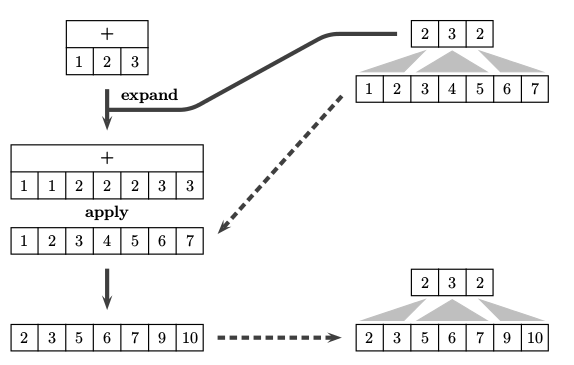
\includegraphics[width=\linewidth]{mapP.png}
        \caption{Conceptional programmer view and actual implementation of \c{mapP (mapP incr)}
        \footnote{Here, the commas in-between the elements have been omitted for visual clarity.
        This thesis will sometimes use such spaces for separation
        instead of commas.
        }
        }
        \label{figure:mapP}
        \end{center}
    \end{figure}
    
    This is the key insight in NDP. Nested parallel functions are
    transformed into calls of \c{mapPL} which avoids the nesting of
    the arrays entirely and maps over the array is a single pass.
    Using this procedure, one can transform nested data parallel programs
    to flat data parallel programs. The former is easier to write in and flexible
    - while the latter can be implemented directly and is efficient.
            
    Vectorization itself is a complex transformation and many details were omitted.
    More details can be found in \cite{Harness2008}.
    
  \subsection{Communication Fusion}
    During Communication Fusion
    \footnote{as described in
    \cite{DistTypes1999} and \cite{TypesNested2000}
    }
    lifted functions like \c{incrL} are inlined.
    They generally have following form:
    \begin{lstlisting}
incrL :: PA Int -> PA Int
incrL = joinD . mapD incrS . splitD
    \end{lstlisting}
    The types of the new functions are explained in \ref{mapPs}.
    Essentially, the lifted functions are implemented by explicitly
    splitting the array across all PUs (\c{splitD}), applying the original
    function (in this case \c{incrS}) on each local chunk sequentially (\c{mapD})
    and finally joining all chunks {\c{joinD}}.
    
    The type \c{Dist a} denotes a distributed value of type \c{a}.
    Distributable values can for example be arrays or linked lists.
    In case of arrays, the array is chunked and distributed evenly.
    In case of linked lists, the lists is chunked and
    inter-PU pointers are used when each chunk reaches its end.
    
    Another aspect to note is the following distinction:
    The use of \c{PA a} means, that the entire array
    is processed by a single PU locally and
    then redistributed globally to all PUs.
    The use of \c{Dist a} means,
    that each PU is processing its
    chunk of the distributed value locally.
    
    After these introducing words, one can take a look at the type of expressions
    Communication Fusion is designed to optimise. Here is an example.
    \begin{lstlisting}
myFunc :: PA Int -> PA Int
myFunc = mult2L . incrL
    \end{lstlisting}
    where \c{mult2L} is a function which doubles each element in the array.
    Currently, the function works in two steps. Applying the operations individually.
    First, it splits the array, increments its elements and joins the array. Second, it splits
    the array again, doubles its elements and rejoins the array.
    A more efficient alternative would execute both operations locally
    in a single pass rather than two. The compiler needs optimisations.
    
    Effective optimisation strategies in referentially transparent
    programming languages like Haskell are \emph{Inlining}
    \footnote{\cite{Inlining2002}}
    and \emph{Rewrites Rules}
    \footnote{\cite{Simon2001Rewrites}}
    .
    Inlining refers to the inlining of definitions
    of functions and variables. Inlining the definitions
    of the functions in the snipper reveal the following:
    \begin{lstlisting}
myFunc :: PA Int -> PA Int
myFunc = joinD . mapD mult2S . splitD . joinD . mapD incrS . splitD
    \end{lstlisting}
    Then rewrite rules are used. They allow the specification of general semantic-preserving
    laws and allow the compiler to rewrite parts of the code according to them.
    They are written by humans and table \ref{rules} introduces some of them.
    Among them is "splitD/joinD". It states the general law,
    that joining and re-splitting an array does not change the array at all.
    This is clear for humans - but not for the compiler. By specifying such rules
    the compiler is aided in optimising the code.
    In our case the compiler finds the splitD/joinD pair and applies the rule to get:
    \begin{lstlisting}
myFunc :: PA Int -> PA Int
myFunc = joinD . mapD mult2S . mapD incrS . splitD
    \end{lstlisting}
    The was able to eliminated communication in-between two phases of computation.
    This is a step towards more efficient evaluation.
    Using another rule, namely "mapD/mapD", the compiler can further optimise to.
    \begin{lstlisting}
myFunc :: PA Int -> PA Int
myFunc = joinD . mapD (mult2S . incrS) . splitD
    \end{lstlisting}
    Communication Fusion did not only reduce the communication but also
    packed together consecutive operations. This is desirable behaviour.
    Now the compiler can further optimise local operations using Stream Fusion.
    
  \subsection{Stream Fusion}
    Stream Fusion concerns the optimisation of recursive composed functions
    into a single loop. It is a complex topic
    \footnote{A few papers on Stream Fusion:
    \cite{GenVectorFusion2013}, \cite{Fusion2007},
    \cite{ArrayFusion2001Chakravarty}
    and \cite{CostArray2002Leshchinskiy}
    } and this section will give a broad overview.
    For the purposes of this thesis it is sufficient to state the following:
    \begin{itemize}
      \item Stream Fusion is applied similarly to Communication Fusion.
      \item Instead of inlining \c{fooL} functions, the \c{fooS} functions are inlined.
      \item Instead of mergeing "splitD/joinD", pairs of "unstream/stream" are merged.
      \item Instead of joining "mapD/mapD", pairs of "mapS/mapS" are joined.
      \item \c{Stream a} is a special stream-full data structure.
        Functions over streams are implemented non-recursively.
        They are crucial for the Stream Fusion.
      \item Any streams left over after optimisations are converted back into.
        \c{Vector a}. Streams are only used for optimisation, but not as a collection.
    \end{itemize}
    Applying Stream Fusion creates the following code:
    \begin{lstlisting}
myFunc :: PA Int -> PA Int
myFunc = joinD . mapD (mapS (mult2 . incr)) . splitD
    \end{lstlisting}
    In contrast to the prior - two step - distributed computation,
    the new function has been optimised to reduce communication
    and applies both operations in a single loop per PU.
    
  \subsection*{Functions and Rewrite Rules}
    The transformation in chapter \ref{chapter:ndpv} is going to
    make use of many functions. Most common ones are explained in table \ref{mapPs}.
    The table also holds for other functions with same suffix - e.g.
    the \c{mapP} row similarly applies to \c{scanlP}, \c{groupP} etc.
    
    \begin{table}[h!]
      \caption{Overview of Functions and Phases in NDP}
      \label{mapPs}
      \begin{tabular}{lll}
          \toprule
          function & first appearance/ & type/ \\
            & execution context & description \\
          \midrule
          mapP f xs & Programer-view & \type{(a -> b) -> [:a:] -> [:b:]} \\
           & not executed & \textbf{P}arallel array functions the programer uses \\
          mapPS f xs & Vectorization & \type{(a -> b) -> PA a -> PA b} \\
           & not executed & \textbf{P}arallel \textbf{S}calar functions over flat arrays \\
          indexPL is xs & Vectorization & \type{PA Int -> PA (PA a) -> PA a} \\
           & not executed & \textbf{P}arallel \textbf{L}ifted indexing on flat arrays. It's scalar\\
           & & function is \type{indexP :: Int -> [:a:] -> a} \\
          mapD f x & Communication Fusion & \type{(Vector a -> Vector b)} \\
           & mapD: all PUs & \type{ -> Dist (PA a) -> Dist (PA b)} \\
           & & Each PU applies \c{f} on it's chunk of the \\
           & f: local per PU & \textbf{d}istributed value. True parallelsim here! \\
          fooS f xs & Communication Fusion & \type{Vector a -> Vector b}\\
           & local PU & Applies a function \textbf{s}equentially. \\
           & & \c{Vector} is the Haskell implementation of \\
           & & conventional PU-local in-memory arrays. \\
          splitD & Communication Fusion & \type{PA -> Dist (PA a)}\\
           & all PUs & splits a glboal array into chunks and \\
           & & distributes them to each of the PUs \\
          joinD & Communication Fusion & \type{Dist (PA a) -> PA a} \\
           & allPUs & join a distributed array into a global array \\
          stream & Stream Fusion & \type{Vector a -> Stream a}\\
           & not executed & convert from an array to a stream-ful data container \\
          unstream & Stream Fusion & \type{Stream a -> Vector a}\\
           & not executed & convert back to an array \\
          mapSt f xs & Stream Fusion & \type{(a -> b) -> Stream a -> Stream b}\\
           & not executed & Applies a function on a \textbf{st}ream of values \\
      \end{tabular}
    \end{table}

    \nomenclature{\c{Vector}}{is the Haskell implementation of conventional local in-memory arrays.
            They are used as the distributed chunks of \pad.}
    
    Most of the functions are simply inlined during optimisation.
    They do not exist at runtime anymore and
    therefore they are marked 'not-executed'.
    Besides these functions, the compiler needs rewrite rules.
    Most important ones are described in table \ref{rules}.
    
    \begin{table}[h!]
      \caption{Rewrite Rules in NDP}
      \label{rules}
      \begin{tabular}{lll}
          \toprule
          rule & rewrite & description \\
          \midrule
          splitD/joinD & splitD . joinD = id & Joining and splitting an distributed array  \\
          & & is equivalent to a no-op. \\
          
          mapD/mapD & mapD g . mapD f & Two consecutive mappings are \\
          & = mapD (g . f) & equivalent to a single mapping \\
          & & with both of the functions \\
          
          mapD/replD & mapD f . replD n & Replicating a value and mapping \\
          & = replD n . f & all values is equivalent to \\
          & & directly applying the function and \\
          & & subsequently replicating it. \\
          
          splitD/replPS & splitD . replPS n & Replicating and splitting a value \\
          & = replD n & is equivalent to creating the local chunks\\
          & & directly. ReplD implements this and knows \\
          & & which chunk its PU is responsible for. \\
          
          ZipReplSplit & zipWithD f (replD a) & Zipping with a replicated value\\
          & . splitD  & already in scope - is equivalent to - applying \\
          & = mapD (f a) & the mapping with the value \\
          & & curried into the function.\\
          
          mapD/zipWithD & mapD f . zipWithD g xs = & A map operation after a zip operation \\
          & zipWithD (\lam x y -> f (g x y)) xs & is equivalent to a single zip operation \\
          & & that applies both \c{f} and \c{g}. \\
          
          unstream/stream & unstream . stream = id & Converting back and fourth is \\
          &  & equivalent to doing nothing. \\
       \end{tabular}
    \end{table}
  
  \subsection*{A word on accuracy}
    The project of NDP in Haskell is - even after 15 years -
    still in \textit{work in progress}. Due to frequent changes,
    the source papers use conflicting notation and refer to
    different statuses of progress. Inconsistent literature and a project
    still in work is a problem for a thesis on that topic.
    It is not simple to use the original ideas from NESL directly
    on Haskell as there are great differences in-between them (not mentioning
    the 15 years of research already in it).
    
    Therefore, in this thesis, the author has improvised on a few conflicting or
    missing details to create an overall consistent view on NDP.
    The author specifically used implementations which could really have been
    used in NDP.\footnote{E.g. \c{groupP} as introduced in chapter \ref{chapter:ndpn} does not
    is not included in NDP right now. However, its implementation described there is perfectly possible.}
    The reader is hereby noted that the details
    mentioned here are implementable - but not necessarily an accurate
    representation of the current state of progress.
    
    After this introduction to NDP, the next sections will explain
    parallel complexitiy measures and \algo.
  
\section{Parallel Complexity Measures}
  \label{section:parmeasures}
  In Parallel Computing, the notion of time complexity
  has to be revisited. The time complexity becomes dependent on the
  number of processors available.
  
  Two key measures of an algorithm are \emph{work} complexity
  and \emph{depth} complexity. Work is defined
  to be the time (counted in number of operations)
  the algorithms needs, if it were executed on a single processor.
  Depth is defined as the longest chain of sequential data dependency.
  It is also the time needed if one had an unlimited number of processors.
  
  There are limited ways to calculate work and depth. Both are defined
  recursively over the work and depths of their sub-expressions. Generally,
  work is the sum of operations involved in all of the sub-expressions
  - while depth is the maximum of number of operations involved in
  any particular chain of sub-expressions.
  In this thesis, the functions $\W(\cdot)$ and $\D(\cdot)$ denote work
  and depth, respectively. In some cases, syntactic constructs
  like $\W(f,x)$ are used to denote the work involved in \emph{applying}
  \c{f} on \c{x}. It does not include the work involved
  in calculating \c{x} in the first place. Sometimes,
  the thesis denotes $\W(n)$ or $\D(n,gmax)$ to emphasize,
  that the work and depth is dependent of the length of the input
  or of the parameter $gmax$. In these cases, the function referred to
  is clear from the context.
  Table \ref{table:workdepth} gives work and depth complexities the parallel primitives
  of table \ref{table:parfuns}.
  
  \begin{table}[h]
    \caption{Work and Depth - Definitions and Complexities}
    \label{table:workdepth}
    \begin{center}
    \begin{tabular}{lll}
      \toprule
      function & work & depth \\
      \midrule
      g . f & $\W(g) + \W(f)$ & $\D(g) + \D(f)$ \\
      mapP f xs & 1 + $\W(xs) + \sum_{x \in xs}\W(f,x)$ & 1+ $\D(xs) + \max_{x \in xs}\D(f,x)$ \\
      zipWith f as bs & 1 + $\W(as) + \W(bs)$ & 1 + $\D(as) + \D(bs)$ \\
        & $+ \sum_{pairs (x,y) \in (xs,ys)}\W(f,x,y)$ & $ + \sum_{pairs (x,y) \in (xs,ys)}\D(f,x,y)$ \\
      sortP & $O(n \log n)$ & $O(\log n)$ \\
      sumP & n & $\log$ n \\
      replP &  n & 1 \\
      (!:),indexP & 1 & 1 \\
      lengthP & 1 & 1 \\
      headP & 1 & 1 \\
      lastP & 1 & 1 \\
      concatP & 1 & 1 \\
      unconcatP & 1 & 1 \\
    \end{tabular}
    \end{center}
  \end{table}
  
  The work and depth of \c{mapP} embodies the idea, that both are the sum or maximum of the sub-expressions.
  
  An example is given now. Given the expression
  \c{ys = mapP inrc (replP n 1)}, one can apply
  the formulas to calculate its work and depth complexity.
  \begin{equation*}
  \begin{split}
  \W(ys)
        & = 1 + \W(replP,n,1) + \sum_{x \in xs}\W(incr,x) \\
        & = 1 + n + n \\
        & \in O(n) \\
  \D(ys) & = 1 + \D(replP,n,1) + \max_{x \in xs}\D(incr,x) \\
      & = 1 + 1 + 1 \\
      & \in O(1) \\
  \end{split}
  \end{equation*}
  $xs$ is the intermediate array created by \c{replP}.
  The expression has constant depth - and therefore
  is expected to be executable in constant time if given enough processors.
  If one had as many PUs as the array is in size
  - one could assign each PU one element of the array and process
  the elements locally. Each PU would execute a constant number of operations
  This is indeed constant time in total.
  
  These measures, as introduced in \cite{Belloch1996}, work
  neatly within Nested Data Parallelism. Consider for example the
  expression \c{mapP (mapP incr) ass} where the
  nested array \c{ass} has dimensions $w \times h$.
  Within NDP, the nested parallel expression is flattened into a
  flat array and mapped over once only.
  Therefore, work of $O(w \cdot h)$ and depth of $O(1)$ are expected.
  This is indeed the result.
  \begin{equation*}
  \begin{split}
  \W(mapP,mapP,incr)
        & = 1 + \sum_{as \in ass}\W(mapP,incr,as) \\
        & = 1 + \sum_{as \in ass}(1 + \sum_{a \in as} \W(incr,a)) \\
        & = 1 + \sum_{as \in ass}(1 + \sum_{a \in as} 1) \\
        & = 1 + \sum_{as \in ass}(1 + h) \\
        & = 1 + w \cdot (1 + h) \\
        & \in O(w \cdot h) \\
  \D(mapP,mapP,incr) & = 1 + \max_{as \in ass}\D(mapP,incr,as) \\
        & = 1 + \max_{as \in ass}(1 + \max_{a \in as} \D(incr,a)) \\
        & = 1 + \max_{as \in ass}(1 + \max_{a \in as} 1) \\
        & = 1 + \max_{as \in ass}2 \\
        & = 1 + 2 \\
        & \in O(1) \\
  \end{split}
  \end{equation*}
  
  Work and depth are an useful tool in measuring
  programs complexity. In the remaining thesis,
  the work and depths complexities (mostly without their derivation)
  are presented.
  \comment{
    More detailed derivations of the complexities shown
    in the algorithms sections can be found
    on the appendix.
  }


\section{\algo}
  \label{section:hbalanceintro}
  This section will introduce \algo. It will state the problem and give an overview of its solution.
  
  \subsection*{Problem}
    Suppose an $w \times h$-8-bit-gray-tone image with low contrast.
    \footnote{Photo by Phillip Capper. Source: \url{https://en.wikipedia.org/wiki/File:Unequalized_Hawkes_Bay_NZ.jpg}}
    
    \begin{figure}[h]
      \centering
      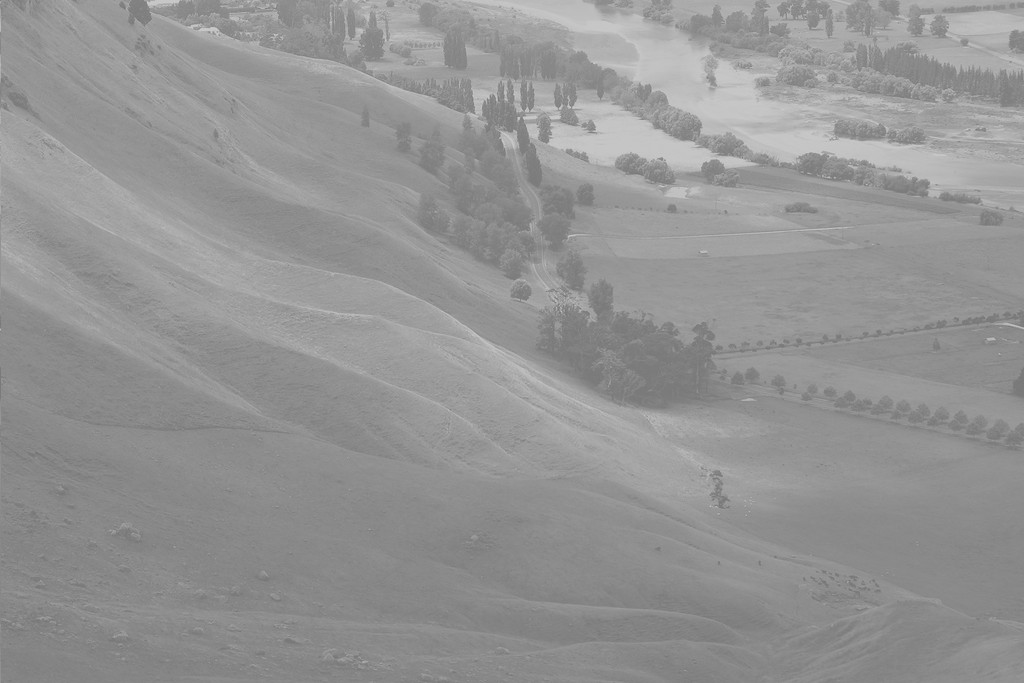
\includegraphics[width=0.45\textwidth]{img-org}
      \caption{An image with low constrast}
      \label{fig:img-org}
    \end{figure}
    The goal is to make details more visible to the human viewer.
    Inspecting the images histogram reveals new insights.
    \footnote{made by used Wikipedia user \c{Jarekt}. Source: \url{https://en.wikipedia.org/wiki/File:Unequalized_Histogram.svg}}
    
    \begin{figure}[h]
      \centering
      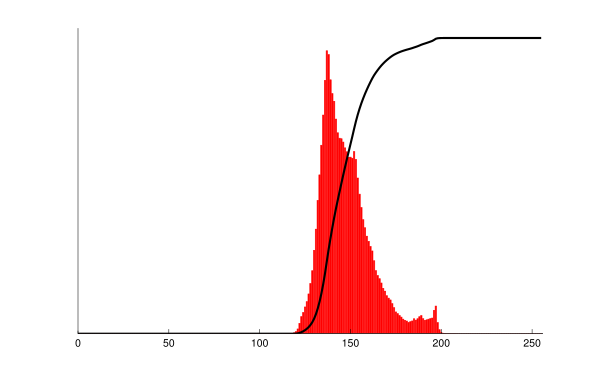
\includegraphics[width=0.45\textwidth]{hist-org}
      \caption{The histogram of the original image with absolute(red) and accumulative(black) count.}
      \label{fig:hist-org}
    \end{figure}
    
    A histogram shows the gray tone distribution of the image.
    The x-axis denotes the gray tone and the y-axis denotes the
    number of pixels with a gray tone $x$ (red). The black curve denotes the
    total number of pixels with a gray tone $g$ such that $g \leq x$.

    Details are difficult to recognize in the original image
    due to their tight packing in the histogram. The
    entire image limits its values to the range [120..205].
    \algo solves this problem by defining a mapping
    $f: Graytone \rightarrow Graytone$, such that the accumulating count
    of the resulting image increases as uniformly as possible from 0 to 255.
    The histogram \ref{fig:hist-eq}
    \footnote{made by used Wikipedia user \c{Jarekt}. Source: \url{https://en.wikipedia.org/wiki/File:Equalized_Histogram.svg}}
    is the envisioned goal.
    
    \begin{figure}[h]
      \centering
      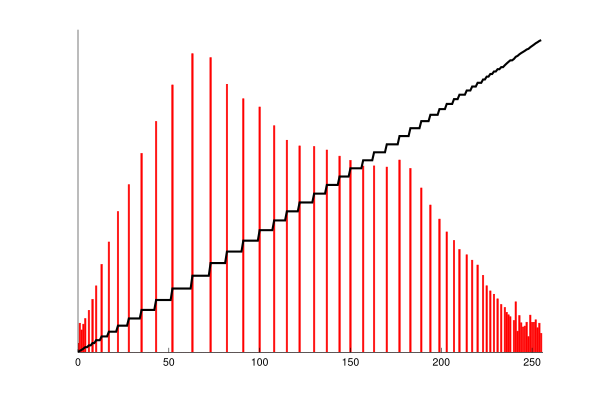
\includegraphics[width=0.45\textwidth]{hist-eq}
      \caption{The histogram of the balanced image}
      \label{fig:hist-eq}
    \end{figure}
    This mapping can be defined by spreading out the gray tones such that more
    frequent gray tones get a larger range to occupy. This idea is
    explained more in detail next.
    \comment{
      Given this interpretation, one can proceed by,
      first build the accumulating histogram (1 and 2) and remembering which
      bar belongs to which gray tone, normalize(3) and scale(4) the bars to [0..255] - 
      and finally - assign each bar (and therefore its gray tone) a new gray tone
      using the bars location in the range [0..255](5).
    }
    % TODO? I should include visual diagrams for this in the thesis.
      
  \subsection*{Algorithm}
    To describe the image transformation $ hbalance: Image \rightarrow Image$ a few definitions are necessary:
    
    \begin{table}[h!]
    \label{table:hbaldefs}
    \centering
    \begin{tabular}{ll}
      $Image$ & := $(Width,Height,Width \times Height \rightarrow Graytone)$ \\
      $Histogram_a$ & $: Graytone \rightarrow a$ \\
      $gmax$ & : $Graytone$ \\
    \end{tabular}
    \end{table}
    
    An $Image$ assigns a gray tone to each pair of coordinates. It is bounded in width and height.
    A $Histogram_a$ assigns a value of type $a$ to each gray tone. For $a = Int$,
    this becomes is an (accumulated) histogram. For $a = Double$, one can
    describe normalised histograms.
    $gmax$ is the maximum gray tone for the gray tones in use (e.g. 255 for 8-bit gray tones).
    
    The method is broken down into the following functions:
      
    \begin{enumerate}
      \item $hist: Image \rightarrow Histogram_{Int}$ \newline
        It calculates the histogram of an image.
      \item $accu: Histogram_{Int} \rightarrow Histogram_{Int}$ \newline
        It calculates the accumulating histogram from the original histogram.
      \item $normalize: Int \times Int \times Histogram_{Int} \rightarrow Histogram_{Double}$  \newline
        It normalizes the accumulated histogram
        to a range from 0 to 1. (3)
        The arguments are denoted $a0$ and $agmax$.
        $agmax$ denotes the number of total pixels in the image.
        $a0$ denoted the number of pixels with the lowest gray tone - namely 0.
        Normalisation is defined in mapping the histogram values by $x \mapsto \frac{(x - a0)}{agmax - a0}$.
        \comment{
          For an accumulated histogram $a:Histogram_{Int}$ it can be calculated with
          $a(gmax)$ or $a(g')$ where $g'$ is highest gray tone in the image.
          Both are equal, so the implementations may take the liberty to use any of these formulas.
        }
      \item $scale: Graytone \times Histogram_{Double} \rightarrow Histogram_{Int}$  \newline
        It scales the normalized values to the maximum gray tone (gmax) and rounds down to the nearest integer.
        Scaling is defined in mapping the histogram values by $x \mapsto \left \lfloor{x \cdot gmax}\right \rfloor $.
      \item $apply: Histogram_{Int} \times Image \rightarrow Image$  \newline
        It maps each gray tone to its new value as dictated by the histogram in the first argument.
    \end{enumerate}
      
    Given these functions $hbalance: Image \rightarrow Image$ can be defined as:
    \begin{equation*}
    \begin{split}
        h & := hist(img) \\
        a & := accu(h) \\
        n & := normalize(a(0), a(gmax), a) \\
        gs & := scale(gmax,n) \\
      hbalance(img) & := apply(gs,img) \\
    \end{split}
    \end{equation*}
    
    Concrete implementations are given in the coming chapters.
    Applying the algorithm to the example image gives \ref{fig:img-eq}
    \footnote{Photo by Phillip Capper. Source: \url{https://en.wikipedia.org/wiki/File:Equalized_Hawkes_Bay_NZ.jpg}}
    . Details are indeed more distinguishable in the balanced image.
    
    \begin{figure}[h]
      \centering
      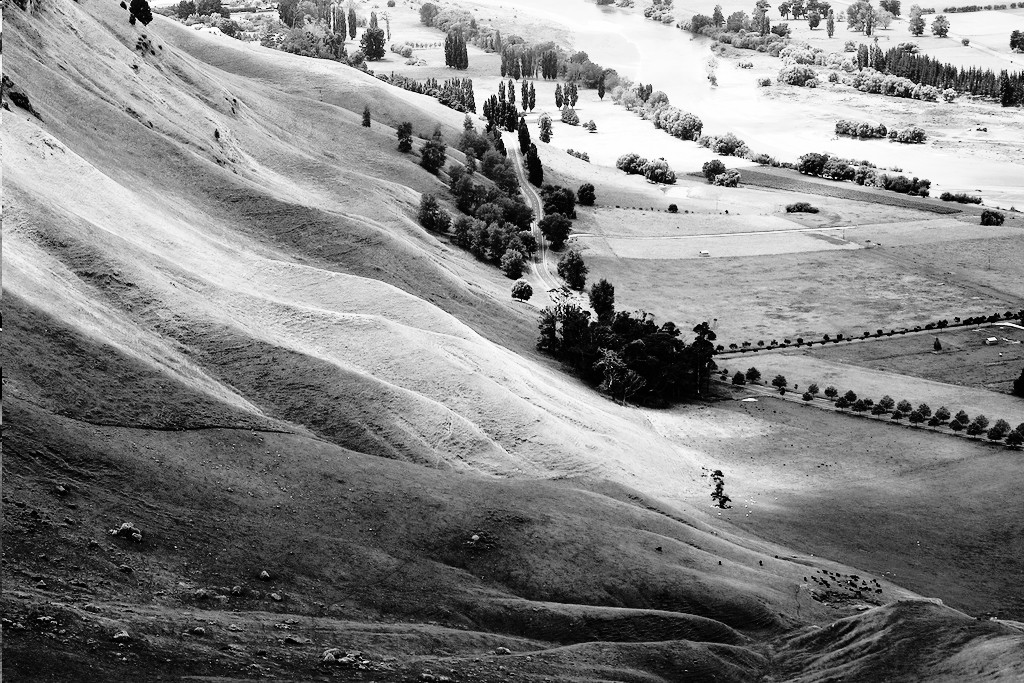
\includegraphics[width=0.45\textwidth]{img-eq}
      \caption{The equalized image}
      \label{fig:img-eq}
    \end{figure}
    
  \algo{} is a frequently used algorithm in image processing. It is 
  one of first methods applied on images to decrease their complexity.
  These balanced images are often then forwarded to sophisticated
  image processing algorithms.
  
  
  \paragraph{}
    The introduction is over and
    the programs \seq, \man\, \ndpn and \ndpv
    are presented and analysed next.
  
  % TODO: cite a book for its uses and the algorithm itself
    
  \comment{
    Prefix sum is a very common operation in computer science. It is a special
      case of scanning through a ordered container from left ro right applying a binary
      associative function \c{f}.
      It is defined as:
        $$ scanl(f,z,[a_1,a_2,...,a_n])
           := [f(z,a_1),f(f(z,a_1),a_2),...,f(f(...f(f(z,a_1),a_2)...,a_{n-1}),a_n)]
        $$
      An example shall be $scanl(+,0,[1,2,2,3,-2]) = [1,3,5,8,6]$. In some definitions
      the first element is $z$. This is however not the definition one needs here.
  }
